% Three slides for the 3-minute presentation, handed in as a 3-page PDF with the paper (no animations).
% Started by Diego with Claude, 22 Nov. Owner: Martin (M8). Compiles in Overleaf as a plain Beamer file:
% upload this file and ../figures/figure1.pdf, figure2.pdf (fix the paths below if you put them elsewhere).
\documentclass[aspectratio=169,11pt]{beamer}
\usetheme{default}
\setbeamertemplate{navigation symbols}{}
\setbeamertemplate{footline}{}
\setbeamerfont{frametitle}{size=\Large,series=\bfseries}
\definecolor{cross}{HTML}{7D3C98}

\begin{document}

% ---------------------------------------------------------------- 1. Question and data
\begin{frame}{Two maps of the same House}
\begin{columns}[T]
\column{0.55\textwidth}
\textbf{Question.} Is the House less divided by party in whom members \emph{name} than in whom they \emph{work
with}?

\vspace{0.6em}
\textbf{Same 450 members, 119th House (2025--26), two records:}
\begin{itemize}
\item \textbf{Working map:} A cosponsors B's bill (govinfo, 46,513 ties)
\item \textbf{Floor map:} A names B in a floor speech (Congressional Record, 9,988 mentions)
\item \textbf{Close-up:} whom members name at home (55,023 press releases)
\end{itemize}
\column{0.42\textwidth}
\vspace{1em}
\textit{Votes and words say Congress is two camps. Does it look the same in who credits whom?}
\end{columns}
\end{frame}

% ---------------------------------------------------------------- 2. The main figure
\begin{frame}{Members name across the aisle more than they work across it}
\centering
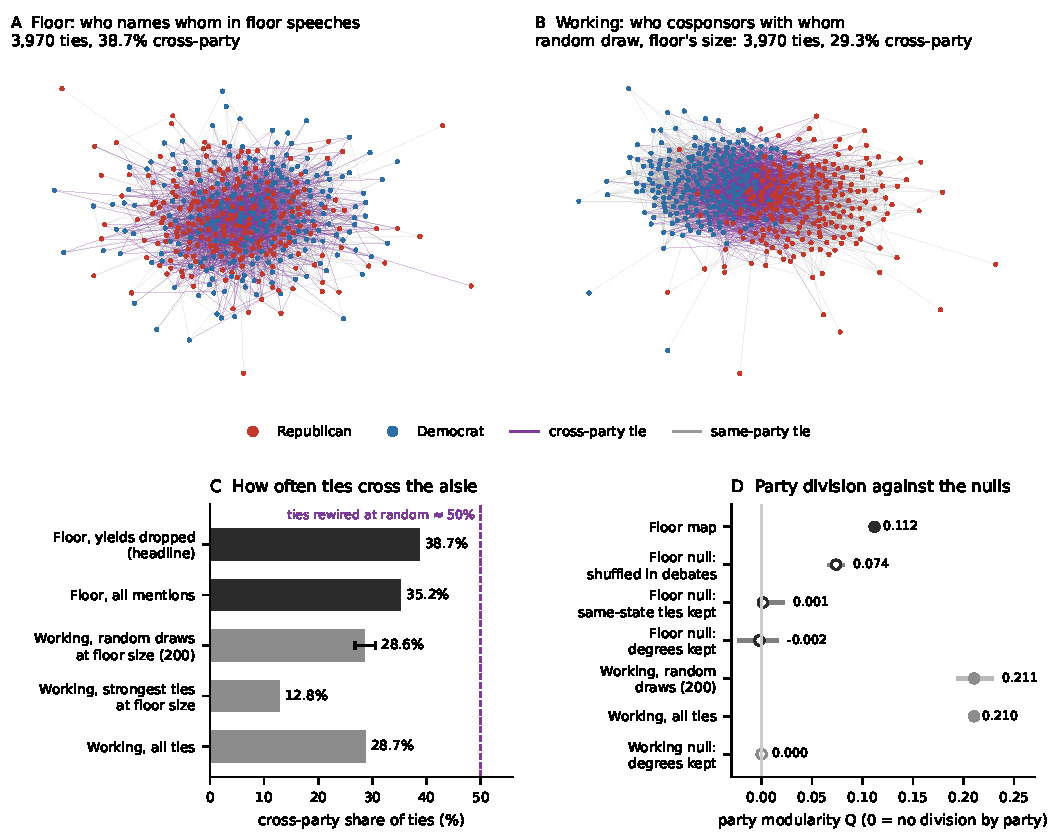
\includegraphics[height=0.68\textheight]{../figures/figure1.pdf}

\vspace{0.3em}
{\Large \textcolor{cross}{\textbf{38.7\%}} of floor ties cross parties, against \textbf{28.6\%} of working ties
of the same size}
\end{frame}

% ---------------------------------------------------------------- 3. What it means and how we checked
\begin{frame}{Mostly credit, not argument; partly procedure}
\begin{columns}[T]
\column{0.5\textwidth}
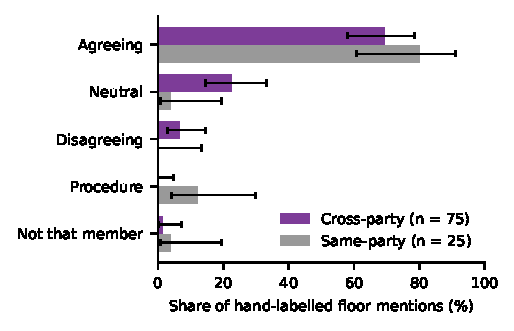
\includegraphics[width=\textwidth]{../figures/figure2.pdf}

\small Cross-party mentions: \textbf{69\% agreeing}, 7\% disagreeing (100 read by hand)
\column{0.48\textwidth}
\textbf{What it means}
\begin{itemize}
\item Members credit colleagues of the other party in public
\item Debate procedure explains about two thirds of the floor map's party division; its communities are committees
\item At home, members in close seats name the other party more (both parties)
\end{itemize}
\textbf{How we checked}
\begin{itemize}
\item Three null models; maps compared at equal size
\item Name matcher: 98/100 right, recall 12/13
\item Two human coders, $\kappa = 0.64$; text classifier did not beat the baseline, so not used
\end{itemize}
\end{columns}
\end{frame}

\end{document}
